%  
% � Mattias Schlenker 
% Dieser Text ist nicht frei, bitte wegen CC-Lizenzierung anfragen!
% 


\documentclass{beamer}
%\usepackage[german]{babel}
% \usepackage[iso-8859-1]{inputenc}
\usepackage[latin9]{inputenc}
\setbeamertemplate{navigation symbols}{}
\usetheme{Warsaw}

\beamersetuncovermixins{\opaqueness<1>{25}}{\opaqueness<2->{15}}
\begin{document}
\title{Mir gen�gt ein Arduino! Microcontroller statt Prozessor}  
\author{Mattias Schlenker}
\date{28. Juni 2014} 

% Titelseite 

\begin{frame}
\titlepage
\end{frame}

% TOC-Seite

\begin{frame}
\frametitle{Inhalt}
\tableofcontents
\end{frame} 

\section{Arduino vs. RaspberryPi} 

\begin{frame}
\frametitle{Worin unterscheiden sich die beiden Bastlerplatinen?} 
Auf den ersten Blick bietet der Raspberry Pi mehr als 1000 mal soviel Rechenleistung wie ein Arduino Uno f�r zehn Euro Aufpreis. Da f�llt die Entscheidung leicht, oder?

Sehen wir uns die Unterschiede doch einmal n�her an:
\end{frame}

\subsection{Technische Daten}
\begin{frame}
\frametitle{Speicher und Rechenleistung} 
\begin{tabular}{c c c c}
\textbf{Plattform} & \textbf{Arduino} & \textbf{Raspberry Pi} & \textbf{Faktor} \\ 
\pause 
RAM/Variablenspeicher & 2048 & 536870912 & 262144\\
\pause 
Festspeicher & 32768 & 8589934592 & 262144 \\
\pause 
,,Rechenleistung'' (MIPS) &  16 & ~ 1000 & 64 \\
\end{tabular} 
\end{frame}

\begin{frame}
\frametitle{IO und Buses}
Arduino heisst in diesem Kontext Atmega328P, Raspberry Pi meint das Model B...
\newline

\begin{tabular}{c c c c}
\textbf{Plattform} & \textbf{Arduino} & \textbf{Raspberry Pi} & \textbf{Faktor} \\ 
\pause
GPIO digital & 17 & 8 & unfair! �pfel vs Birnen! \\
\pause
analog & 6 & 0 & 0 \\
\pause
SPI & 1 & 2 & 2 \\
\pause
UART (seriell) & 1 & 1 & 1 \\
\pause
I2C & 1 & 1 & 1 \\
\end{tabular} 
\end{frame}

\begin{frame}
\frametitle{Interrupts} 
Arduino heisst in diesem Kontext Atmega328P, Raspberry Pi meint das Model B...
\newline

\begin{tabular}{c c c c}

\textbf{Plattform} & \textbf{Arduino} & \textbf{Raspberry Pi} & \textbf{Faktor} \\ 
\pause
Steigend/Fallend & 2 & 8? Publikum? & ? \\
\pause
Wakeup-Timer & 2 & beliebig viele & ? \\
\end{tabular} 

\end{frame}

\begin{frame}
\frametitle{Leistungsaufnahme} 

Arduino heisst in diesem Kontext Atmega328P, Raspberry Pi meint das Model B...
\newline

\begin{tabular}{c c c c}

\textbf{Plattform} & \textbf{Arduino} & \textbf{Raspberry Pi} & \textbf{Faktor} \\ 
\pause
\textbf{ohne Optimierungen} & 40mA bei 5V & 300mA bei 5V & 7,5 \\
\pause
\textbf{optimiert} & 4$\mu$A bei 3,0V & 60mA bei 3,6V & 15000 \\
\pause
\end{tabular}

\begin{itemize}
\item Optimierungen beim Arduino: BOD abschalten, ADC abschalten, Tiefschlaf, Batteriebetrieb mit 2xAAA, Takt auf 8MHz reduziert.
\item Optimierungen beim Raspberry Pi: Abschalten nicht ben�tigter Schnittstellen, Aufl�ten eines optimierten Spannungswandlers, Akkubetrieb mit 3,6V.
\end{itemize}

\end{frame}

\begin{frame}
\frametitle{Preise} 
 
 Auf den ersten Blick liegen Arduino und Raspberry Pi preislich eng beieinander. Auf den zweiten Blick:
 
\begin{itemize}
\item Raspberry Pi: 35 bis 40 \euro
\pause
\item Arduino Uno oder Zero: 25 bis 30 \euro
\pause
\item Arduino Pro Mini (Sparkfun oder Watterott): 10 \euro
\pause
\item Arduino Pro Mini (China-Klon): 3 bis 4 \euro
\pause
\item Atmega328P im DIL28-Geh�use: 3 bis 5 \euro
\end{itemize}

\end{frame}

\subsection{Einsatzbereiche}

\begin{frame}
\frametitle{Arduino} 
\begin{itemize}
\item \emph{Energiesparende} Sensoren oder Aktoren: Jahrelanger Betrieb auf zwei AAA-Zellen m�glich
\item \emph{Billige} Sensoren: Totalverlust ist zu verschmerzen
\item \emph{Billige} Peripherie: Der integrierte ADC erlaubt den Anschluss von Thermistoren statt One-Wire-Temperatursensoren
\item \emph{einfache} Sensoren und Aktoren: auch gr��ere St�ckzahlen (Sensornetze, Kunstprojekte) lassen sich mit wenigen Bauteilen schnell fertigen
\end{itemize}
\end{frame}

\begin{frame}
\frametitle{Raspberry Pi} 
\begin{itemize}
\item \emph{Billige} Basis f�r Sensornetze
\item \emph{Stromsparende} ,,Au�enstelle'': Solarbetrieb mit relativ kleinem Panel m�glich
\item \emph{Gro�e} Flexibilit�t dank ,,normalem'' Linux
\end{itemize}

\end{frame} 
\section{Die Arduino-Zukunft}

\begin{frame}
\frametitle{Quo Vadis, Arduino?}

Die Arduino-Familie f�cherte in den letzten Jahren immer mehr auf. Ein deutlicher Trend sind Platinen, die wie der Raspberry unter Linux laufen? Werden sie dem RPi gef�hrlich? Entfremdet sich Arduino von seiner urspr�nglichen Zielgruppe?

\end{frame}

\subsection{,,Starke'' Arduinos mit Linux}

\begin{frame}
\frametitle{Galileo}

Intel verschenkt an Unis Galileo-Boards im Arduino-Shield-Layout. Das besondere: Statt Microcontroller kommt ein Pentium zum Einsatz:

  \begin{center}
    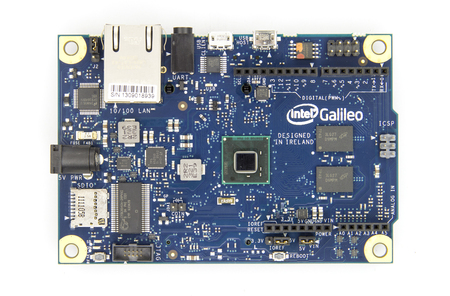
\includegraphics[width=8cm]{photos/galileo.jpg}
  \end{center}
\end{frame}

\begin{frame}
\frametitle{Galileo}

Intel verschenkt an Unis Galileo-Boards im Arduino-Shield-Layout. Das besondere: Statt Microcontroller kommt ein Pentium zum Einsatz:
\newline

\begin{itemize}
\item Intels Versuch, mit Embedded x86 in die N�he von Microcontrollern zu kommen
\item Referenzboard f�r Intels Quark SoC x1000
\item Arduino-Code wird in ELF-Objekte kompiliert
\item recht langsames IO
\item \emph{Mattias' Meinung:} The worst of both worlds
\end{itemize}
\end{frame}

\begin{frame}
\frametitle{Arduino Tre}
Gemeinsam mit TI und dem BeagleBone-Projekt entwickelter ,,janusk�pfiger'' Arduino aus TI Sitara und Atmega32u4, Leistung der Linux-Seite h�her als beim Raspberry Pi:

  \begin{center}
    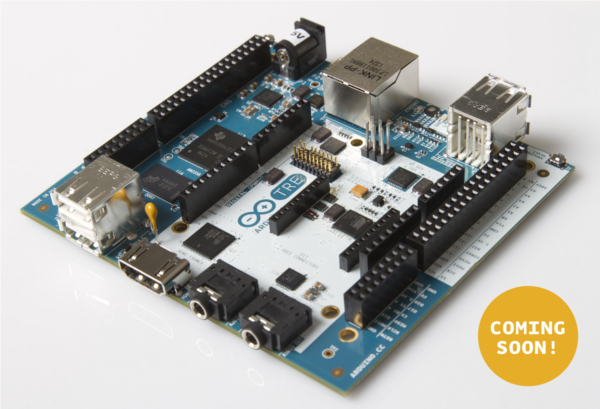
\includegraphics[width=8cm]{photos/arduinotre.jpg}
  \end{center}
\end{frame}

\begin{frame}
\frametitle{Arduino Tre}
Gemeinsam mit TI und dem BeagleBone-Projekt entwickelter ,,janusk�pfiger'' Arduino aus TI Sitara und Atmega32u4, Leistung der Linux-Seite h�her als beim Raspberry Pi:

\begin{itemize}
\item Von TI als Referenzplattform betrachtet
\item 100\% Code-Kompatibilit�t zu Arduino Leonardo
\item 100\% Code-Kompatibilit�t zu Beaglebone Black
\item recht teuer - Entwicklerkit 149 \euro - final 60 bis 80 \euro
\item \emph{Mattias' Meinung:} Tolles Konzept, hohe Leistung, aber hoher Preis und gro�e Platine
\end{itemize}
\end{frame}

\begin{frame}
\frametitle{Arduino Y�n}
Janusk�pfiger Arduino aus MIPS-Prozessor und Atmega32u4, Formfaktor des Uno, Leistung der Linux-Seite deutlich kleiner als beim Raspberry Pi, daf�r incl. WLAN und schnell angebundenem Ethernet:

  \begin{center}
    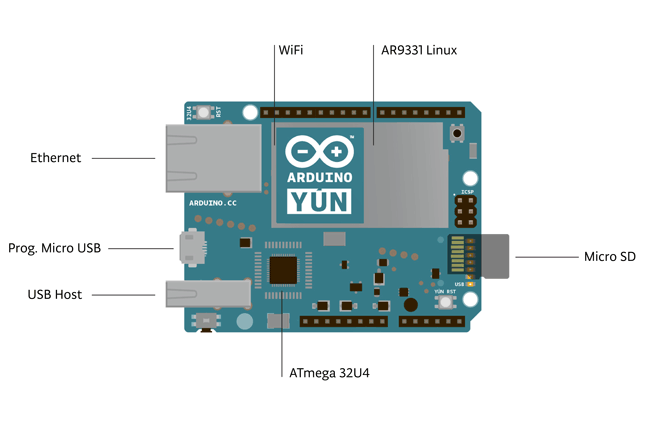
\includegraphics[width=8cm]{photos/YunParts.png}
  \end{center}
\end{frame}

\begin{frame}
\frametitle{Arduino Y�n}
Janusk�pfiger Arduino aus MIPS-Prozessor und Atmega32u4, Formfaktor des Uno, Leistung der Linux-Seite deutlich kleiner als beim Raspberry Pi, daf�r incl. WLAN und schnell angebundenem Ethernet:
\newline

\begin{itemize}
\item Eigenentwicklung mit Fokus auf guter Nutzbarkeit
\item 100\% Code-Kompatibilit�t zu Arduino Leonardo
\item OpenWRT basierte Distribution f�r die MIPS-Seite
\item Stra�enpreis 60 bis 75 \euro - kann parallel als WLAN Access Point genutzt werden
\item \emph{Mattias' Meinung:} Tolles Konzept, passende Leistung, sollte etwas g�nstiger sein
\item \emph{Der Clou:} Die Software - einfacher geht es nicht!
\end{itemize}
\end{frame}

\begin{frame}
\frametitle{Arduino Y�n - Software-Integration}
Eine neue Sammlung von Bibliotheken f�r die Arduino-IDE abstrahiert die Kommunikation zwischen Microcontroller- und Microprozessorseite:
\newline

\begin{itemize}
\item Bridge-Bibliothek f�r Zugriff auf viele Netzwerkfunktionen aus Arduino-Sketches - nur eine Programmiersprache n�tig!
\item ,,Mailbox'' (toter Briefkasten) f�r den Datenaustausch zwischen Microcontroller und Microprocessor
\item Integration von Temboo - abstrahiert verschiedene Webdienste
\item Voller Paketumfang von OpenWRT
\item Einfaches Webinterface f�r die Einrichtung - Luci bekannt von OpenWRT
\end{itemize}
\end{frame}

\begin{frame}
\frametitle{Arduino Y�n - Twitter-Beispiel}
  \begin{center}
    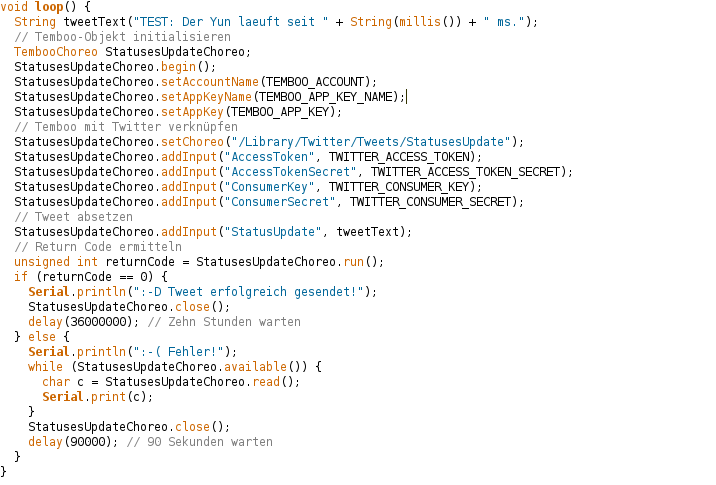
\includegraphics[width=10cm]{photos/codetwitter.png}
  \end{center}
\end{frame}

\begin{frame}
\frametitle{Arduino Y�n - Tweets ganz praktisch}
  \begin{center}
    
\includegraphics[width=9cm]{photos/tweet.png}
  \end{center}

Wozu? ,,Horst von Forst'', unser Weihnachtsbaum twitterte, wenn er zuwenig Wasser hatte. Der vollst�ndige Code und Erkl�rungen zum verwendeten Sensor unter: http://www.arduino-hausautomation.de/
\end{frame}

\subsection{Neue Microcontroller mit ARM-Kern}

\begin{frame}
\frametitle{Arduino Due}
Erstes Arduino-Board mit 32Bit-ARM-Microcontroller. Ca. 45 \euro. CAN-Interface. Blick in die Zukunft ohne weitere Relevanz. Daher keine technischen Details:

  \begin{center}
    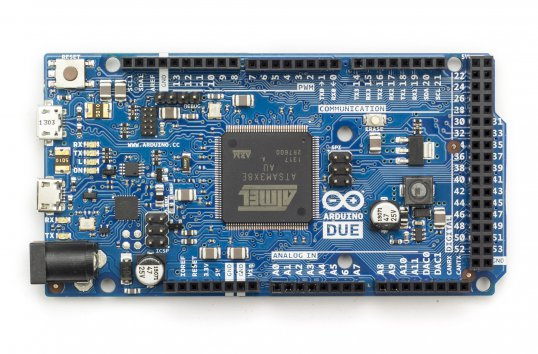
\includegraphics[width=8cm]{photos/arduinodue.jpg}
  \end{center}
\end{frame}

\begin{frame}
\frametitle{Arduino Zero}
Designierter Nachfolger des Arduino Uno mit SAMD21G18, h�here Integration verspricht g�nstigere Preise:

  \begin{center}
    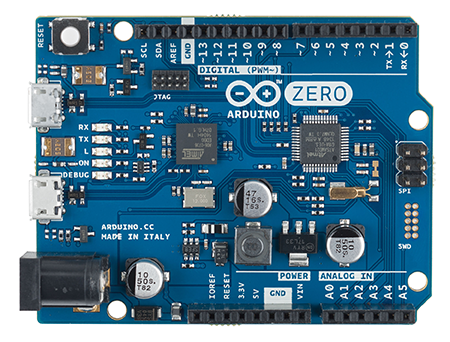
\includegraphics[width=8cm]{photos/arduinozero.png}
  \end{center}
\end{frame}

\begin{frame}
\frametitle{Arduino Zero}
Designierter Nachfolger des Arduino Uno mit SAMD21G1, h�here Integration verspricht g�nstigere Preise:
\newline 

\begin{itemize}
\item 32 Bit Microcontroller mit ARM-Kern
\item 256kB Flash 
\item 32kB SRAM 
\item Hohe Integration mit Debugger und 2xUSB
\item Tendenziell Preise auf Level von Atmega32u4 oder Atmega328P - kleine Klone f�r weniger als 5 \euro\  m�glich
\item \textbf{Achtung!} 3,3 Volt
\item \textbf{Achtung!} kein DIL Package des Controllers erh�ltlich
\end{itemize}

\end{frame}

\subsection{Problem Fragmentierung}

\begin{frame}
\frametitle{Bitte unterbrechen!}

\textbf{Falls Mattias in diesem Abschnitt ausschweift, bitte unterbrechen!}

\end{frame}


\begin{frame}
\frametitle{Microcontroller-Familien von Arduino}

Im Laufe der Jahre wurden von Arduino immer mehr Microcontroller-Familien unterst�tzt, nicht nur kleine Spr�nge wie von Atmega168 auf Atmega328, sondern mehrere Br�che. Offizielle Familien:
\newline

\begin{itemize} 
\item Atmega328: Arduino Uno, Pro Mini
\item Atmega32u4: Leonardo, Y�n, Micro
\item Atmega2560: Mega2560
\item \emph{neu} ATSAMD21: Arduino Zero, Due
\item \emph{neu} Intel Galileo - noch nicht eingepflegt in Arduino IDE
\end{itemize}
\end{frame}

\begin{frame}
\frametitle{Kompatibilit�tsprobleme}

Daraus ergeben sich Kompatibilit�tsprobleme, beispielsweise wenn Code von einem Microcontroller auf den anderen portiert werden soll:

\begin{itemize} 
\item Spannungsunterschiede: Mal 3,3V, mal 5V
\item Unterschiedliche Position der Pins f�r SPI
\item Code zum extremen Energiesparen ist Controllerspezifisch
\item Viele Bibliotheken unterst�tzen bislang nur 328 und 32u4
\end{itemize}
\end{frame}

\begin{frame}
\frametitle{Hoffnung?}
Kann der ARM-Kern die Fragmentierung stoppen?

\begin{itemize} 
\item Abl�sung der 32u4 basierten Controller durch ARM
\item Fokus der Entwickler schnell auf ARM?
\item Atmega328P wird noch eine Weile bleiben (DIL-Package!)
\item Andere Controllerhersteller werden zu Arduino sto�en 
\item Billige Klone im Mini-Format machen Verlust der DILs wett
\item Arduino wird offener und emanzipiert sich von Atmel
\end{itemize}
\end{frame}




\section{Gemeinsam stark!}

\subsection{Raspberry Pi mit Arduino huckepack}

\begin{frame}
\frametitle{Das Problem}

Raspberry Pi ist billig und leistungsstark, aber:
\newline

\begin{itemize}
\item Viele Bibliotheken nur f�r Arduino erh�ltlich
\item Hoher Aufwand, Bibliotheken und Protokolle zu portieren
\item Keine analogen Ports
\end{itemize}
\end{frame}

\begin{frame}
\frametitle{Die L�sung}

Wir kombinieren einfach Raspberry Pi und Arduino:
\newline

\begin{center}
\textbf{Best of both worlds!}
\end{center}

\begin{itemize}
\item Alle Arduino-Bibliotheken nutzbar
\item GPIO des Raspberry bleibt erhalten
\item Weniger als 10 Euro Investition
\end{itemize}
\end{frame}

\begin{frame}
  \begin{center}
    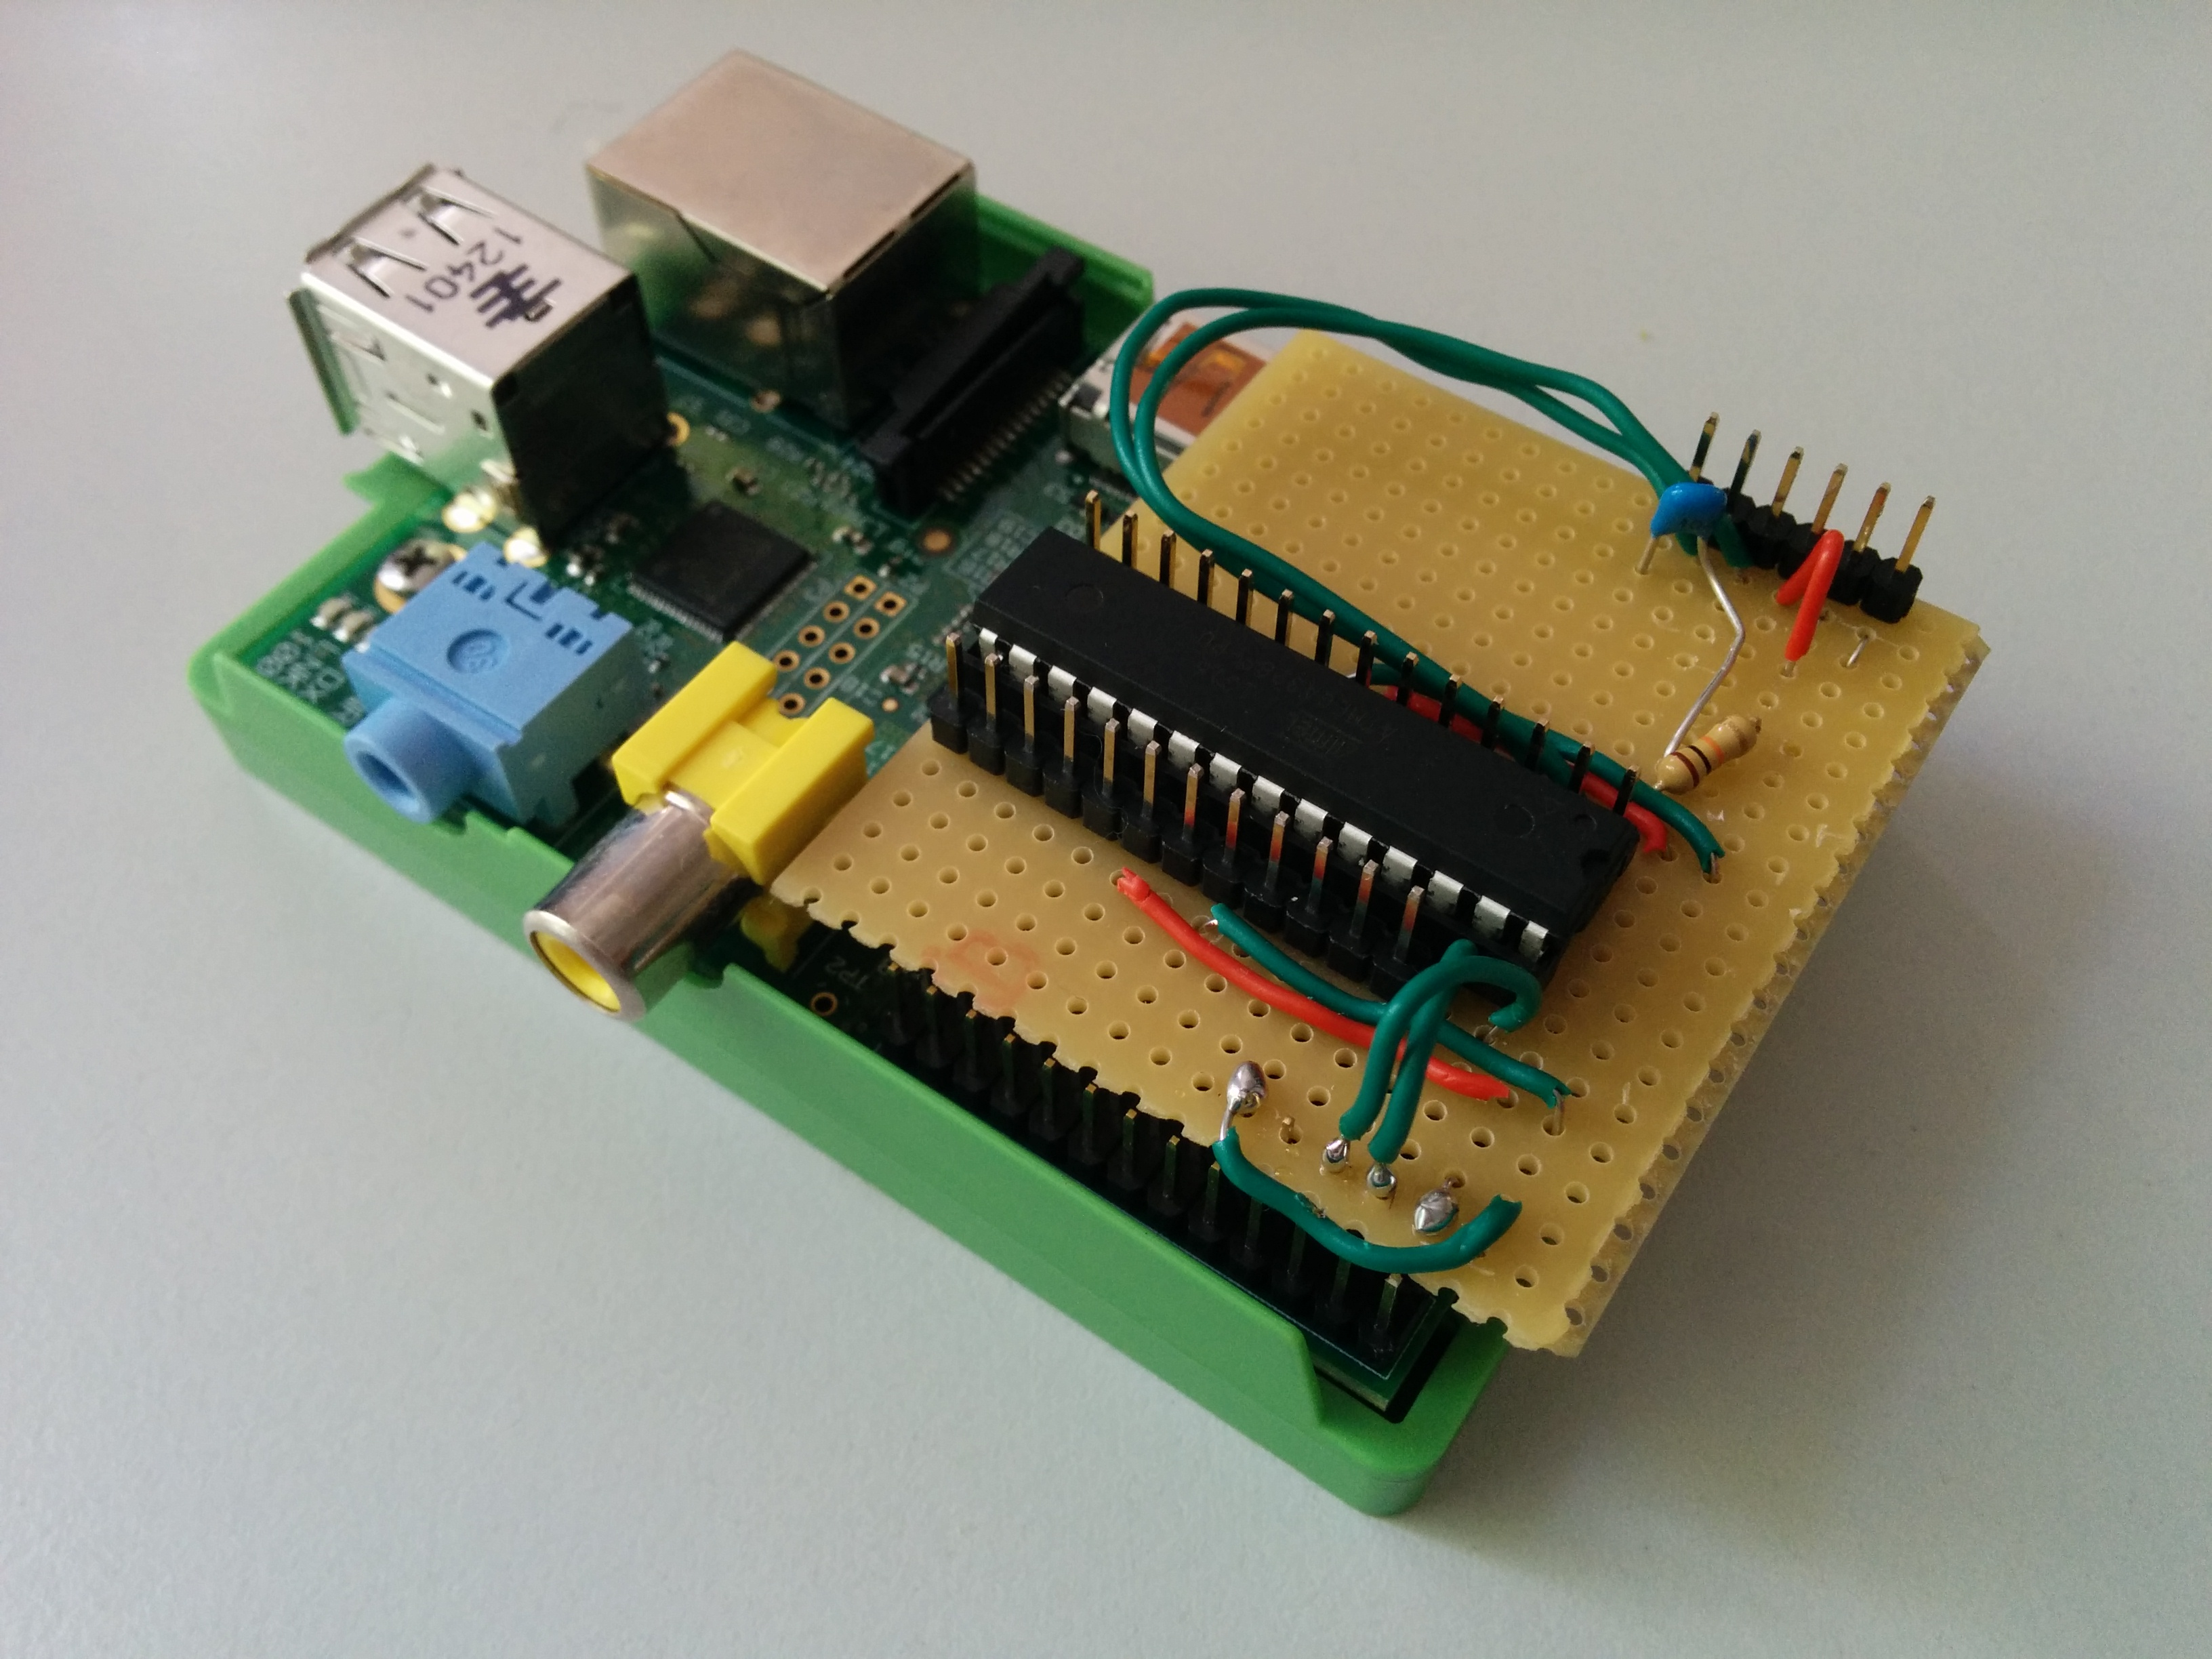
\includegraphics[width=10cm]{photos/IMG_20140623_144020.jpg}
  \end{center}
\end{frame}


\begin{frame}
\frametitle{Und wie geht das?}

\begin{itemize}
\item Nackter Atmega328P huckepack
\item Spannungsversorgung durch 3,3V-Schiene des Raspberry
\item Kommunikation �ber I2C-Bus - weitere Bus-Teilnehmer m�glich
\item \textbf{Bonus:} Atmega328P kann direkt vom Raspberry Pi programmiert werden
\end{itemize}
\end{frame}


\begin{frame}
\frametitle{Beispielcode Arduino}
  \begin{center}
    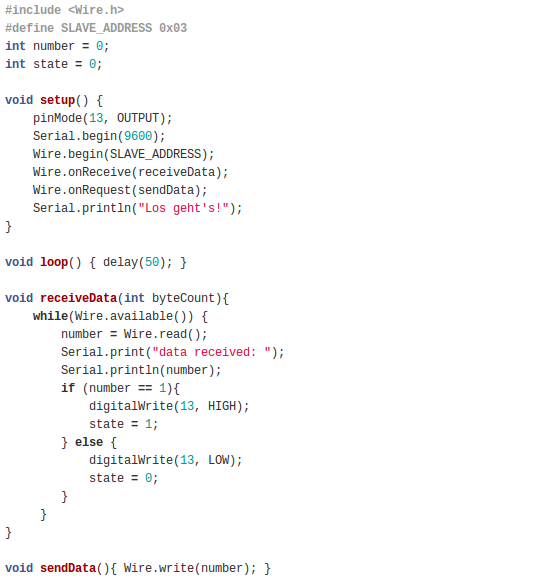
\includegraphics[width=6.3cm]{photos/i2carduino.png}
  \end{center}
\end{frame}

\begin{frame}
\frametitle{Beispielcode Raspberry}
  \begin{center}
    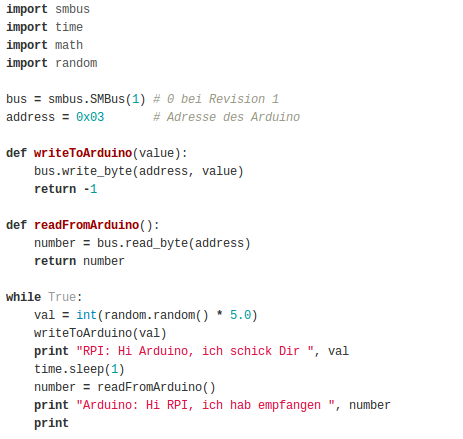
\includegraphics[width=6.3cm]{photos/i2craspberry.png}
  \end{center}
\end{frame}

\begin{frame}
\frametitle{Vor- und Nachteile}
\textbf{Vorteile}
\begin{itemize}
\item Billig: Atmega328P gibt es in der Fuzo beim blauen C
\item Schnell realisiert
\item Sehr flexibel
\end{itemize}

\textbf{Nachteile}
\begin{itemize}
\item Zwei Sprachen involviert: Python und Arduino
\item Kein fertiges Protokoll: Handarbeit angesagt
\item Nur bei 3,3V-Betrieb bleiben alle Vorteile von I\textsuperscript{2}C erhalten
\end{itemize}

\end{frame}

\subsection{Raspberry Pi als Zentrale}

\begin{frame} 
\frametitle{Kommunikation �ber's Netz}
Arduinos mit Enc28J60-Ethernetmodul kommunizieren mit dem Raspberry Pi:
\newline

\begin{itemize}
\item UDP-Kommunikation bei Arduino simpel realisierbar
\item UDP-Empfang auf Raspberry-Seite nur wenige Zeilen Python
\item Billige Hardware am Arduino (3 bis 5 \euro \ f�r Enc28J60) 
\item Weniger Einschr�nkungen bei Busl�nge gg�. direktem Onewire
\end{itemize}


\end{frame}
\section{Fazit} 

\begin{frame} 
\frametitle{�pfel mit Birnen vergleichen lohnt nicht!}
\begin{itemize}
\item Verschiedene Tools f�r verschiedene Zwecke
\item Kenntnisse beider Tools helfen, das richtige auszuw�hlen
\item Wer intensiv bastelt, muss kombinieren
\item Konvergenz verwirrt gelegentlich  - leider auch die Hersteller (siehe Galileo!)
\item Kommt r�ber auf die andere Seite!
\end{itemize}
\end{frame}

\begin{frame} 
\frametitle{Revolutionkunde}
\begin{itemize}
\item Arduino: 2004 - die Microcontroller-Revolution
\item Raspberry Pi: 2012 - die Microprocessor-Revolution + Popularisierung von Linux
\end{itemize}

\begin{center}
\textbf{Beides zusammen: Die Maker-Revolution!}
\end{center}
\end{frame}

\begin{frame} 
\frametitle{Danke f�r die Aufmerksamkeit}
\begin{itemize}
\item Mattias Schlenker - \texttt{ms@mattiasschlenker.de}
\item Fork me on Github! \texttt{https://github.com/mschlenker}
\item Webseite \texttt{https://www.arduino-hausautomation.de/}
\item Google+ \texttt{https://plus.google.com/+MattiasSchlenker1}
\end{itemize}
\end{frame}

%\begin{frame}\frametitle{unnumbered lists}
%\begin{itemize}
%\item Introduction to  \LaTeX  
%\item Course 2 
%\item Termpapers and presentations with \LaTeX 
%\item Beamer class
%\end{itemize} 
%\end{frame}

%\begin{frame}\frametitle{lists with pause}
%\begin{itemize}
%\item Introduction to  \LaTeX \pause 
%\item Course 2 \pause 
%\item Termpapers and presentations with \LaTeX \pause 
%\item Beamer class
%\end{itemize} 
%\end{frame}

%\subsection{Lists II}
%\begin{frame}\frametitle{numbered lists}
%\begin{enumerate}
%\item Introduction to  \LaTeX  
%\item Course 2 
%\item Termpapers and presentations with \LaTeX 
%\item Beamer class
%\end{enumerate}
%\end{frame}

%\begin{frame}\frametitle{numbered lists with pause}
%\begin{enumerate}
%\item Introduction to  \LaTeX \pause 
%\item Course 2 \pause 
%\item Termpapers and presentations with \LaTeX \pause 
%\item Beamer class
%\end{enumerate}
%\end{frame}

%\section{Section no.3} 
%\subsection{Tables}
%\begin{frame}\frametitle{Tables}
%\begin{tabular}{|c|c|c|}
%\hline
%\textbf{Date} & \textbf{Instructor} & \textbf{Title} \\
%\hline
%WS 04/05 & Sascha Frank & First steps with  \LaTeX  \\
%\hline
%SS 05 & Sascha Frank & \LaTeX \ Course serial \\
%\hline
%\end{tabular}
%\end{frame}


%\begin{frame}\frametitle{Tables with pause}
%\begin{tabular}{c c c}
%A & B & C \\ 
%\pause 
%1 & 2 & 3 \\  
%\pause 
%A & B & C \\ 
%\end{tabular} 
%\end{frame}

%\section{Section no. 4}
%\subsection{blocs}
%\begin{frame}\frametitle{blocs}

%\begin{block}{title of the bloc}
%bloc text
%\end{block}

%\begin{exampleblock}{title of the bloc}
%bloc text
%\end{exampleblock}

%\begin{alertblock}{title of the bloc}
%bloc text
%\end{alertblock}
%\end{frame}

%\section{Section no. 5}
%\subsection{split screen}

%\begin{frame}\frametitle{splitting screen}
%\begin{columns}
%\begin{column}{5cm}
%\begin{itemize}
%\item Beamer 
%\item Beamer Class 
%\item Beamer Class Latex 
%\end{itemize}
%\end{column}
%\begin{column}{5cm}
%\begin{tabular}{|c|c|}
%\hline
%\textbf{Instructor} & \textbf{Title} \\
%\hline
%Sascha Frank &  \LaTeX \ Course 1 \\
%\hline
%Sascha Frank &  Course serial  \\
%\hline
%\end{tabular}
%\end{column}
%\end{columns}
%\end{frame}

%\subsection{Pictures} 
%\begin{frame}\frametitle{pictures in latex beamer class}
%\begin{figure}
% \includegraphics[scale=0.5]{PIC1} 
%\caption{show an example picture}
%\end{figure}
%\end{frame}

%\subsection{joining picture and lists} 

%\begin{frame}
%\frametitle{pictures and lists in beamer class}
%\begin{columns}
%\begin{column}{5cm}
%\begin{itemize}
%\item<1-> subject 1
%\item<3-> subject 2
%\item<5-> subject 3
%\end{itemize}
%\vspace{3cm} 
%\end{column}
%\begin{column}{5cm}
%\begin{overprint}
%\includegraphics<2>{PIC1}
%\includegraphics<4>{PIC2}
%\includegraphics<6>{PIC3}
%\end{overprint}
%\end{column}
%\end{columns}
%\end{frame}

%\subsection{pictures which need more space} 
%\begin{frame}[plain]
%\frametitle{plain, or a way to get more space}
%\begin{figure}
% \includegraphics[scale=0.5]{PIC1} 
%\caption{show an example picture}
%\end{figure}
%\end{frame}

\end{document}
